\section*{Materiali}

I materiali che abbiamo utlizzato per questa esperienza di laboratorio sono:

\begin{itemize}
    \setlength{\itemsep}{0.5pt}
    \item{Alimentatore di tensione continua, con tensione massima di 50 V.}
    \item{Multimetro digitale.}
    \item{Oscilloscopio.}
    \item{Diodi 1N4007 con tensione di breakdown di 1000 V.}
    \item{Cella fotovoltaica di silicio cristallino.}
    \item{Lampada per illuminare la cella fotovoltaica.}
    \item{Cavi a banana, breadboard e altri cavi di collegamento}
\end{itemize}

\section*{Circuito}

I circuiti utilizzati durante questa sessione di laboratorio sono i seguenti:

\begin{figure}[h]
    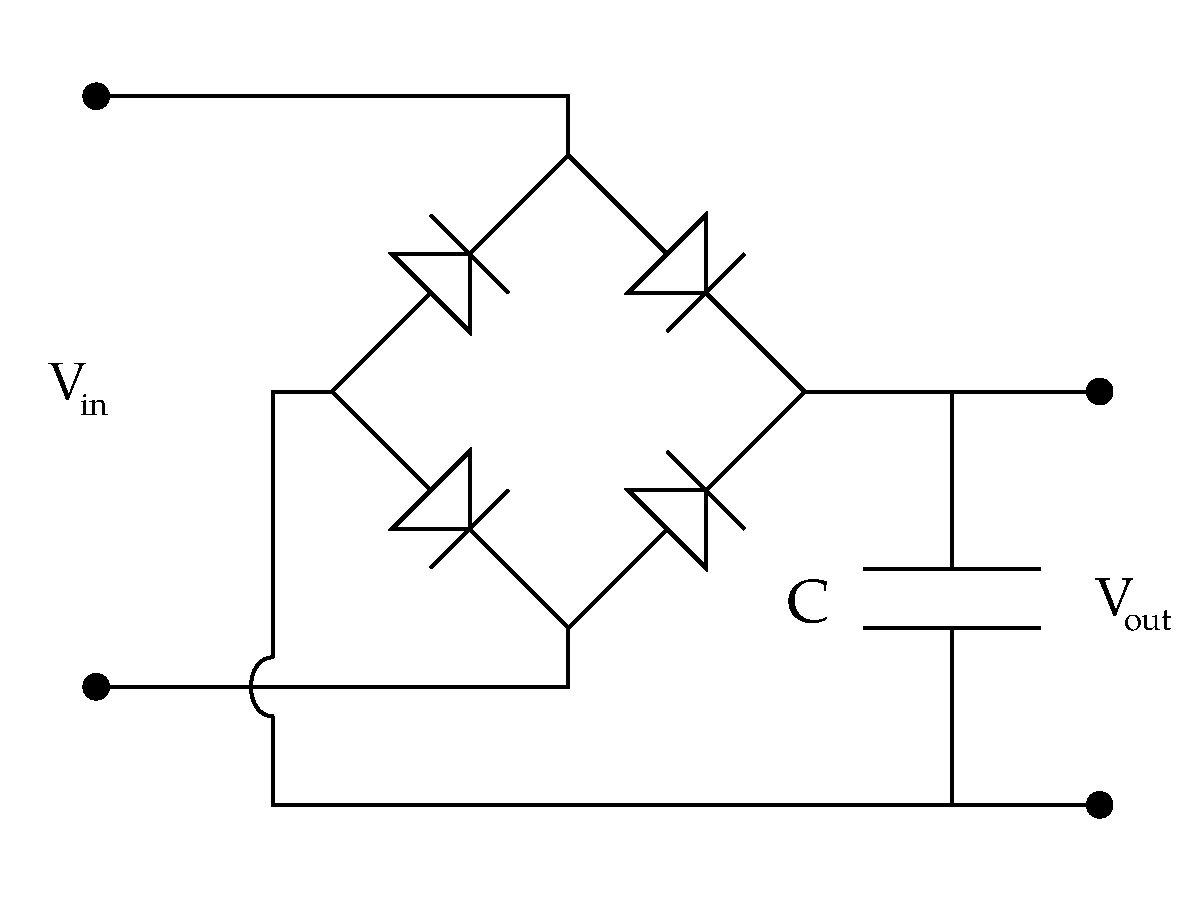
\includegraphics[width=8cm]{graetz.pdf}
\end{figure}
